\documentclass[12pt, letter]{article}
\usepackage{mathptmx}
\usepackage{titlesec}
\usepackage{graphicx}
\usepackage{graphics}
\usepackage{ragged2e}
\usepackage{setspace}
\usepackage[toc, page]{appendix}
\usepackage{amssymb, amsmath}
\usepackage{import}
\usepackage{svg}
\usepackage{xcolor}
\usepackage{siunitx}
\usepackage{caption}
\usepackage{subcaption}
\usepackage{booktabs}
\usepackage{listings}
\usepackage[hidelinks]{hyperref}
\usepackage{xcolor}
\usepackage{longtable,tabularx}
\usepackage[bottom=25mm, top=25mm, left=20mm, right=20mm]{geometry}
\usepackage{pdfpages}
\usepackage{multirow}
\usepackage{fancyhdr}
\usepackage{subcaption}
\usepackage{tocloft}
\usepackage{float}
\usepackage{verbatim}
\usepackage{minted}
\hypersetup{
    colorlinks=true,
    linkcolor=black,
    filecolor=magenta,      
    urlcolor=cyan,
    pdfpagemode=FullScreen,
}
\setstretch{1.1}
%

%%%%%%%%%%%%%%%%%%%%%%%%%%%%%%%%%%%%%%%%%%%%%%%%%%%%%%%%%%%%%%%%%%%%%%%%%%%%%%%%%%%%%%%%%%
%               FORMATTING FOR PRE TECHNICAL CONTENT              %
%%%%%%%%%%%%%%%%%%%%%%%%%%%%%%%%%%%%%%%%%%%%%%%%%%%%%%%%%%%%%%%%%%%%%%%%%%%%%%%%%%%%%%%%%%

\titleformat{\section}
  {\normalfont\centering\sffamily\bfseries}{\thesection}{1em}{}

% Change the style for Table of Contents, Figures and Tables
\renewcommand{\cfttoctitlefont}{\sffamily\large\bfseries}
\renewcommand{\cftloftitlefont}{\sffamily\large\bfseries}
\renewcommand{\cftlottitlefont}{\sffamily\large\bfseries}


%%%%%%%%%%%%%%%%%%%%%%%%%%%%%%%%%%%%%%%%%%%%%%%%%%%%%%%%%%%%%%%%%%%%%%%%%%%%%%%%%%%%%%%%%%
%               BEGINNING OF DOCUMENT              %
%%%%%%%%%%%%%%%%%%%%%%%%%%%%%%%%%%%%%%%%%%%%%%%%%%%%%%%%%%%%%%%%%%%%%%%%%%%%%%%%%%%%%%%%%%
\begin{document}
%%%%%%%%%%%%%%%%%%%%%%%%%%%%%%%%%%%%%%%%%%%%%%%%%%%%%%%%%%%%%%%%%%%%%%%%%%%%%%%%%%%%%%%%%%
%               TITLE PAGE              %
%%%%%%%%%%%%%%%%%%%%%%%%%%%%%%%%%%%%%%%%%%%%%%%%%%%%%%%%%%%%%%%%%%%%%%%%%%%%%%%%%%%%%%%%%%
\begingroup
\let\newpage\relax 
\title{Term Project\\ \Huge{\textbf{OrbitSim}}}
\vspace{200pt}
\date{April 17, 2024}
\maketitle
\thispagestyle{empty}
\endgroup 

\vspace{90pt}
\begin{center}
  \author{\vspace{10pt} Paramvir Singh Lobana \\ Jian Jiao \\ }
\end{center}
\vspace{120pt}
\begin{center}

\includegraphics[scale=0.04]{figures/logo.png}
\end{center}
\begin{center}
\large Department of Mechanical, Industrial and Aerospace Engineering, \\ Concordia University \\ Montreal, QC, Canada
\end{center}
\clearpage
%%%%%%%%%%%%%%%%%%%%%%%%%%%%%%%%%%%%%%%%%%%%%%%%%%%%%%%%%%%%%%%%%%%%%%%%%%%%%%%%%%%%%%%%%%


\pagenumbering{roman}
\tableofcontents

\addcontentsline{toc}{section}{List of Figures}

\pagebreak
\listoffigures
\pagebreak

%%%%%%%%%%%%%%%%%%%%%%%%%%%%%%%%%%%%%%%%%%%%%%%%%%%%%%%%%%%%%%%%%%%%%%%%%%%%%%%%%%%%%%%%%
% This is for adding headers and footers
%\input{header_foorter.tex}

%%%%%%%%%%%%%%%%%%%%%%%%%%%%%%%%%%%%%%%%%%%%%%%%%%%%%%%%%%%%%%%%%%%%%%%%%%%%%%%%%%%%%%%%%%
%               FORMATTING FOR TECHNICAL CONTENT              %
%%%%%%%%%%%%%%%%%%%%%%%%%%%%%%%%%%%%%%%%%%%%%%%%%%%%%%%%%%%%%%%%%%%%%%%%%%%%%%%%%%%%%%%%%%

\titleformat{\section}
  {\large\centering\sffamily\bfseries}{\thesection}{1em}{}
\titleformat{\subsection}
  {\normalfont\sffamily\bfseries}{\thesubsection}{1em}{}
\titleformat{\subsubsection}
  {\normalfont\sffamily\bfseries}{\thesubsubsection}{1em}{}
%%%%%%%%%%%%%%%%%%%%%%%%%%%%%%%%%%%%%%%%%%%%%%%%%%%%%%%%%%%%%%%%%%%%%%%%%%%%%%%%%%%%%%%%%
% DO NOT CHANGE ANYTHING BEFORE THIS IN THE CODE
\pagenumbering{arabic}
\setcounter{page}{1}
%%%%%%%%%%%%%%%%%%%%%%%%%%%%%%%%%%%%%%%%%%%%%%%%%%%%%%%%%%%%%%%%%%%%%%%%%%%%%%%%%%%%%%%%%

\section{Introduction}

Orbital mechanics is a branch of celestial mechanics that focuses on the motion of objects in space under the influence of gravitational forces. It's a fascinating field that explains how satellites, spacecraft, planets, moons, and other celestial bodies move and interact within their orbits. 

The objective of this project is to program and simple self contained orbit simulation software for simulating the motion of satellites. The program is based on C++ language with SFML library to produce a user friendly interface.

The SFML (Simple and Fast Multimedia Library) is a cross-platform software development library designed to provide a simple interface for multimedia tasks such as graphics rendering, window management, audio playback, and user input handling. It's is widely used to create interactive applications. The library is open-source and easily accessible. For this reason it is used to construct the Graphics and improve the interactivity of the software.

The software enables user to manually control the orbit of the satellite by manually initiate prograde and retrograde burns or initiate Hohmann transfer between circular orbits. The software provide instant feedback on the radius and velocity of the satellite and it's orbit condition through the vis-viva equation.

This software is based on simple two body assumption and uses equations covered in the lectures; at the core, the software is an physics based real time simulation. The position of the velocity of the satellite is governed by kinematics and is calculated after each frame. This allows the trajectory of the satellite to be altered by user input instantaneously. However, this method also introduces errors during the calculation and will be discussed in detail in the error sections.

It is envisioned that this software can be used for teaching and live demonstration of simple orbital mechanics as it allows user to see the effect on orbit of their input. It is hoped this software can be a teaching tool for the future students of AERO 485. 


\clearpage





\section{Theories and Assumptions}

\subsection{Assumptions}
    To construct the simulation environment, certain assumptions are made to simplify the governing equations and reduce the complexity of the program. the details of each are discussed below.
\subsubsection {Two Body Universe}
	The gravitational force interaction between the gravity source and the satellite is the only driving force experienced by the satellite. When simulating multiple satellites at one given occasion, the gravitational interaction between the satellite body is ignored.
\subsubsection {2D Planar Assumption}
	The system is programmed in the 2D frame to reduce the computation power required of the program.  
\subsubsection {System Reference}
	A fixed absolute reference system is placed on the gravity source; the gravity source is assumed to be always stationary; thus, the Coriolis effect due to the motion of the gravity source is ignored.
\subsubsection {Instant delta V Application}
	In the simulation, the application of delta V for orbit transfer is applied to the satellite instantly. Although this is not feasible for real life rocket systems to perform such an operation, it provides the best adherence to the Hohmann transfer assumption.



\subsection{Methods and Calculations} \label{sec:theory}
This section covers the equations used to construct the governing equations used in the software.
\subsubsection {System kinematics}
The base function of the software is to simulate the motion of a satellite around a single gravity source in real time, the basic motion of the body is governed by newton’s first law and gravitational law. As the simulation is conducted in 2D frame; only X and Y axis are established for computation.
To compute the position and velocity of the satellite, a cartesian coordinate system is used to describe the position of the satellite. To reduce the complexity, the gravity source is placed at the center of the coordinate system. The position of the satellite then can be described as:
\begin{equation} \label{eq:position}
P_s (x,y)
\end{equation}
The velocity of the satellite than can be written as
\begin{equation} \label{eq:velocity}
V_{s2} (u,v)=\frac{(P_{s2} (x,y)-P_{s1} (x,y))}{t}
\end{equation}
For acceleration, at all times, the satellite is subjected to the gravitational pull of the gravity source; by combining the newton’s first law and gravitational law; the acceleration on the satellite can be obtained by the equation below.
\begin{equation} \label{acceleration}
a=-\frac{GM}{r^2}
\end{equation}
Knowing the gravity source is placed at the origin of the coordinate system; the acceleration vector can be broken down to:
\begin{equation} \label{acceleration_x}
a_x=-\frac{GMx}{r^3}
\end{equation}
\begin{equation} \label{acceleration_y}
a_y=-\frac{GMy}{r^3}
\end{equation}
Where:
\begin{equation} \label{r defination}
r=\sqrt{x^2+y^2}
\end{equation}
Using first order direct integration method; assuming the time step is sufficiently small; the velocity and position of the satellite of the next time step then can be written as:
\begin{equation} \label{next step velocity}
V_{s2} (u,v)=V_{s1} (u,v)+a_t(a_x,a_y )\Delta t
\end{equation}
\begin{equation} \label{next step position}
P_{s2} (x,y)=P_{s1} (x,y)+V_{s2}(u,v)\Delta t
\end{equation}


\subsubsection {Satellite initialization}
To initialize the satellite, the position and the velocity of the satellite must be determined. In this software, the satellite is automatically initialized with a circular orbit. The circular orbit is calculated by coupling the centripetal acceleration to gravitational acceleration equation to obtain the orbiting velocity. 
\begin{equation} \label{Orbit velocity 1}
\frac{V^2}{r}=-\frac{GM}{r^2}
\end{equation}
\begin{equation} \label{Orbit velocity 2}
V=\sqrt{\frac{GM}{r}}
\end{equation}
To simplify the initialization process, the satellite is always initialized with counter clockwise rotation on the positive x-axis; thus, the initial condition of the satellite will be: 
\begin{equation} \label{Initial position}
P_{s0} (r_0,0) 
\end{equation}

\begin{equation} \label{Initial velocity}
V_{s0} (0,-\sqrt{\frac{GM}{r_0}})
\end{equation}


\subsubsection {Hohmann Transfer}
The Hohmann transfer function is achieved by the user adjust the target radius of the orbit.  The software will calculate the $\Delta$ V required for switching to or from the elliptical transfer orbit.  
Using the above equation the velocity of the current and target circular orbit $V_{o1}$, $V_{o2}$ can be obtained from the given orbit height. To construct the transfer orbit, the eccentricity of the ellipse can be written as: 
\begin{equation} \label{eccentricity}
e=\frac{(r_a-r_p)}{(r_a+r_p )}
\end{equation}
Where the perigee and apogee distance of the ellipse correspond to the current and target radius of the circular orbit. As the radius to the periapsis is given by:
\begin{equation} \label{periapsis}
r_p=\frac{h^2}{GM(1+e)}
\end{equation}
Where is h is the angular momentum: $ h=\sqrt{GMr} $ for circular orbit; combining the above equations, the velocity of the satellite at any location can be represented by:
\begin{equation} \label{transfer orbit velocity}
V=\sqrt{GM(\frac{2}{r}-\frac{2}{r_a+r_p })}
\end{equation}
At the transfer altitude, the velocity of the satellite will be:
\begin{equation} \label{apogee velocity}
V_{apo}=\sqrt{GM(\frac{2}{r_a}-\frac{2}{r_a+r_p })}
\end{equation}
\begin{equation} \label{perigee velocity}
V_{peri}=\sqrt{GM(\frac{2}{r_p}-\frac{2}{r_a+r_p })}
\end{equation}
The above equation can also be obtained through Vis-Viva equation.

Adapting the equation to the cartesian coordinate established earlier, the velocity of the satellite can be expressed by the equation below:

\begin{equation} \label{eq:velocity_X}
V_x=\frac{x}{r}\sqrt{GM(\frac{2}{r}-\frac{2}{r_a+r_p })}
\end{equation}
\begin{equation} \label{eq:velocity_Y}
V_y=\frac{y}{r}\sqrt{GM(\frac{2}{r}-\frac{2}{r_a+r_p })}
\end{equation}

The $\Delta$ V required for the two operations then can be obtained by:
\begin{equation} \label{eq:Transfer velocity 1}
\Delta V_1=V_{apo}-V_{o1}
\end{equation}
\begin{equation} \label{eq:Transfer velocity 2}
\Delta V_2=V_{s2}-V_{peri}
\end{equation}
For the simulation, when the user initiated the transfer operation, the velocity of the satellite will be updated to the transfer orbit velocity and the perigee and apogee simulate the impulse burn. 


\subsubsection {User Control Consideration}
\noindent \textbf{vis-viva equation}
\begin{equation} \label{eq:visviva}
\epsilon=\frac{V^2}{2}-\frac{GM}{r}
\end{equation}
The vis-viva equation is used to indicate the state of the orbit. The equation is derived based on the energy law to compare the kinetic energy to the gravitational potential. If the initial gravitational energy of the satellite is equal or lower than the kinetic energy; the user will be prompted with the vis-viva result turning red indicating the satellite escaping.

\noindent \textbf{Kepler’s 3rd law}
\begin{equation} \label{eq:kepler3rd}
T=\frac{2\pi}{\sqrt{GM}}a^{\frac{3}{2}}
\end{equation}
where
\begin{equation} \label{eq:semi_major_axis}
a=\frac{2}{\frac{2}{r}-\frac{V^2}{GM}}
\end{equation}

Kepler’s third law is used to compute the period time of the satellite for completing one orbit. The semi-major axis is computed once  based on the vis-viva equation with the current velocity and radius of the satellite. In the software; the period time is calculated in frame rate to make the result independent from the capacity of the computer. the semi-major axis is calculated though the orbit condition.


\clearpage



\section{Design and Development}
The OrbitSim desktop application is developed using C++ programming language. To create the graphical user interface, the SFML graphics library is used. The source code is present in the appendix and the Visual Studio project can be accessed from the following github repository \href{https://github.com/paramvirlobana/SpacePropulsion-W2024}{OrbitSim}.

\subsection{Identified Requirements}
The following are the identified requirements to build an interactive system to observe the satellite.
\begin{enumerate}
    \item \textbf{Function 1:} The user shall be able to manually control the velocity and adjust the orbit of the satellite.
    \item \textbf{Function 2:} The user shall be able to adjust the target orbit radius after the Hohmann transfer.
    \item \textbf{Function 3:} The user shall be able to reset the satellite or normalize the satellite orbit into a circular orbit after manual manipulation of the orbit
    \item \textbf{Function 4:} The user presses `T' to conduct the transfer instantaneously. The console window prompts the user the stage of the transfer. During the transfer all other functions outside normalize and reset are disabled 
    \item \textbf{Function 5:} The user shall be able to zoom in and out of the frame using scroll wheel.
\end{enumerate}

\subsection{Numerical Implementation}
This class ``GravitySource" as seen in \autoref{fig:class_gravity_source}, represents a body with gravitational influence. It stores position and strength parameters, along with graphical attributes. The constructor initializes these properties, setting the position and strength based on input values. It also configures a graphical representation of the celestial body using the SFML library. The render method displays the graphical representation on a given window.

\begin{figure}[H]
    \begin{minted}[frame=lines,fontsize=\footnotesize,linenos]{cpp}
class GravitySource{
	sf::Vector2f pos; sf::Vector2f pos_e;
	float strength;
	sf::CircleShape s; sf::Texture texture_earth;
public:
	GravitySource(float pos_x, float pos_y, float strength){
		pos.x = pos_x; pos.y = pos_y;
		this->strength = strength;
		pos_e.x = pos_x - 30; pos_e.y = pos_y - 30;
		s.setPosition(pos_e);
		s.setRadius(30);
	}
	void render(sf::RenderWindow& wind){
		wind.draw(s);
	}
	sf::Vector2f get_pos(){
		return pos;
	}
	float get_strength(){
		return strength;
	}
};
    \end{minted}
    \caption{Code snippet for the defined gravity source.}
    \label{fig:class_gravity_source}
\end{figure}




The ``Particle" class as seen in \autoref{fig:class_particle} simulates an object in space. It contains position, velocity, and path data, along with methods for rendering and physics updates. The constructor initializes position and velocity. The ``update\_physics" function calculates gravitational acceleration from a given GravitySource, updating velocity and position over time.

\begin{figure}[H]
    \begin{minted}[frame=lines,fontsize=\footnotesize,linenos]{cpp}
class Particle {
	sf::CircleShape s;
	std::vector<sf::Vector2f> path;
public:
	sf::Vector2f pos; sf::Vector2f vel; sf::Vector2f pos_s;
	Particle(float pos_x, float pos_y, float vel_x, float vel_y) {
		pos.x = pos_x; pos.y = pos_y; pos_s.x = pos.x - 6;
		pos_s.y = pos.y - 6;
		vel.x = vel_x; vel.y = vel_y;
		s.setPosition(pos_s); s.setFillColor(sf::Color::Red); s.setRadius(6);
	}
	void render(sf::RenderWindow& wind) {
		s.setPosition(pos_s);
		wind.draw(s);

		for (size_t i = 1; i < path.size(); ++i) {
			sf::Vertex line[] = {
				sf::Vertex(path[i - 1], sf::Color::White),
				sf::Vertex(path[i], sf::Color::White)
			}; wind.draw(line, 2, sf::Lines);
		}}
	void set_color(sf::Color col) {
		s.setFillColor(col);
	}
	void update_physics(GravitySource& s, float dt) {
		float distance_x = s.get_pos().x - pos.x;
		float distance_y = s.get_pos().y - pos.y;

		float distance = sqrt(distance_x * distance_x + distance_y * distance_y);
		float inverse_distance = 1.f / distance;
		float normalized_x = inverse_distance * distance_x;
		float normalized_y = inverse_distance * distance_y;
		float inverse_square_dropoff = inverse_distance * inverse_distance;
		float acceleration_x = normalized_x * s.get_strength() * inverse_square_dropoff;
		float acceleration_y = normalized_y * s.get_strength() * inverse_square_dropoff;
		vel.x += acceleration_x * dt; vel.y += acceleration_y * dt;

		pos.x += vel.x * dt;pos.y += vel.y * dt;
		pos_s.x = pos.x - 6;pos_s.y = pos.y - 6;
		path.push_back(pos);
		if (path.size() > 20000)
			path.erase(path.begin()); // Remove the oldest position
	}
};

    \end{minted}
    \caption{Code snippet for particle class.}
    \label{fig:class_particle}
\end{figure}



\subsubsection{Hohmann Transfer Implementation - Mode 1}
Mode 1 in OrbitSim is the implementation of Hohmann transfers.
The Hohmann transfer is implemented within the code using a three step approach.

\begin{enumerate}
    \item Initialization (i == 0)
    \begin{itemize}
        \item When i equals 0, it indicates the start of the maneuver.
        \item Calculates initial velocity adjustment ($Dv_1$) based on the current altitude ($P_{abs}$) and the target orbit altitude (Target $\_$ O).
        \item Adjusts the particle's velocity to match $Dv_1$, preparing for the transition to the target orbit.
        \item Sets the state (i) to 1 to proceed to the next step.
        \item In the cased of the simulation the gravitation strength is set to 6500.
        \begin{figure}[H]
        \begin{minted}[frame=lines,fontsize=\footnotesize,linenos]{cpp}
        {
        P_abs_tf = P_abs;
        Dv_1 = sqrt(6500 * (2 / P_abs_tf - 2 / (P_abs_tf + Target_O)));
        Dv_2 = sqrt(6500 / Target_O);
        particles[0].vel.x = Dv_1 * V_x / V_abs;
        particles[0].vel.y = Dv_1 * V_y / V_abs;
        i = 1;
        }  
        \end{minted}
        \caption{Code snippet for first burn.}
        \label{fig:class_particle}
        \end{figure}
    \end{itemize}

    \item Transfer (i == 1)
    \begin{itemize}
        \item When i equals 1, it indicates that the initial velocity adjustment has been applied, and the particle is transitioning towards the target orbit.
        \item Checks if the particle's altitude is within a small tolerance (0.1) of the target orbit altitude ($Target_O$).
        \item If the conditions are met, adjusts the particle's velocity to a final adjustment ($Dv_2$) to achieve a stable orbit at the target altitude.
        \item Sets the state (i) to 2 to indicate completion of this step.


        
        \begin{figure}[H]
        \begin{minted}[frame=lines,fontsize=\footnotesize,linenos]{cpp}
        if (-0.1 < P_abs - Target_O && P_abs - Target_O < 0.1 && i == 1){
        particles[0].vel.x = Dv_2 * V_x / V_abs;
        particles[0].vel.y = Dv_2 * V_y / V_abs;
        i = 2;
        }
        \end{minted}
        \caption{Code snippet for the second burn.}
        \label{fig:class_particle}
        \end{figure}
    \end{itemize}


    \item Final Adjustment (i == 2)
    \begin{itemize}
        \item When i equals 2, it indicates that the particle's velocity has been adjusted for stable orbit at the target altitude.
        \item Checks if the particle's altitude is within a very small tolerance (0.01) of the target orbit altitude ($Target_O$).
        \item If the conditions are met, adjusts the particle's velocity to align with the circular orbit at the target altitude.
        \item Sets the state (i) to 3 to complete the maneuver.
        \begin{figure}[H]
        \begin{minted}[frame=lines,fontsize=\footnotesize,linenos]{cpp}
        if (-0.01 < P_abs - Target_O && P_abs - Target_O < 0.01 && i == 2){
	particles[0].vel = sf::Vector2f((P_y - win_y / 2) / P_abs * sqrt(6500 / P_abs),
        -(P_x - win_x / 2) /       P_abs * sqrt(6500 / P_abs));
	i = 3;
        }
        \end{minted}
        \caption{Code snippet for trim error correction.}
        \label{fig:class_particle}
        \end{figure}
    \end{itemize}
    
\end{enumerate}


\subsubsection{User Controlled Burn - Mode 2}
Mode 2 in the OrbitSim desktop applications allows the user to accelerate the body on demand. This is done using the left and right arrow keys on the keyboard. The theory discussed in Section \ref{sec:theory} is used to write the code seen in \autoref{fig:mode_2_1}. \autoref{eq:velocity_X} and \autoref{eq:velocity_Y} are used to write the following part of the code which allows the user to control the particle body trajectory.


\begin{figure}[H]
        \begin{minted}[frame=lines,fontsize=\footnotesize,linenos]{cpp}
    if (sf::Keyboard::isKeyPressed(sf::Keyboard::Left) && i != 0 && i != 1){
    // tangent burn
    particles[0].vel.x += 0.1f * V_x / V_abs;
    particles[0].vel.y += 0.1f * V_y / V_abs;
    i = 10;
    }
    else if (sf::Keyboard::isKeyPressed(sf::Keyboard::Right) && i != 0 && i != 1){
    particles[0].vel.x -= 0.1f * V_x / V_abs;
    particles[0].vel.y -= 0.1f * V_y / V_abs;
    i = 10;
    }
\end{minted}
\caption{Code snippet for user controlled burn.}
\label{fig:mode_2_1}
\end{figure}
\clearpage


Once the user has changed the trajectory, the application also has the functionality to force the particle body into a circular orbit. This is implemented using the code seen in \autoref{fig:mode_2_2}.
\begin{figure}[H]
        \begin{minted}[frame=lines,fontsize=\footnotesize,linenos]{cpp}
    if(sf::Keyboard::isKeyPressed(sf::Keyboard::Space)){
    particles[0].vel = sf::Vector2f((P_y - win_y / 2) / P_abs * sqrt(6500 / P_abs),
    -(P_x - win_x / 2) / P_abs * sqrt(6500 / P_abs));
    i = 3;
    }
\end{minted}
\caption{Code snippet for normalizing current orbit into a circular orbit.}
\label{fig:mode_2_2}
\end{figure}

The graphics and user interface is constructed using the SFML library; the detail of the section can be seen in the appendix.

 \subsection{Graphical Implementation}
 The graphical implementation is done using the SFML library. Different elements are defined within the code, for example real time progress data, static labels/information and graphical images and then rendered on the screen using the draw feature in the SFML library.

\begin{figure}[H]
        \begin{minted}[frame=lines,fontsize=\footnotesize,linenos]{cpp}
    position2.setFont(font);
    position2.setString("position y : " + pos_y_string);
    position2.setCharacterSize(info_char_size);
    position2.setFillColor(sf::Color::Green);
    position2.setPosition(info_x + 220, 800);
    //====================================== DRAW INFORMATION 
    window.draw(position2);
    //===================================== END OF DATA PRINTING 
    window.display();
    t += dt * timeScale;
\end{minted}
\caption{Graphical implementation for rendering the user interface elements}
\label{fig:window_display}
\end{figure}


\clearpage


\section{Results}


\autoref{fig:user_interface} shows OrbitSim’s GUI. The central simulation area visualizes orbital paths, while real-time data such as target radius and normalized position/velocity are displayed on the left. On the right, controls legends allow users to adjust parameters like orbit radius and manage actions such as prograde and retrograde burn.
\begin{figure}[H]
    \centering
    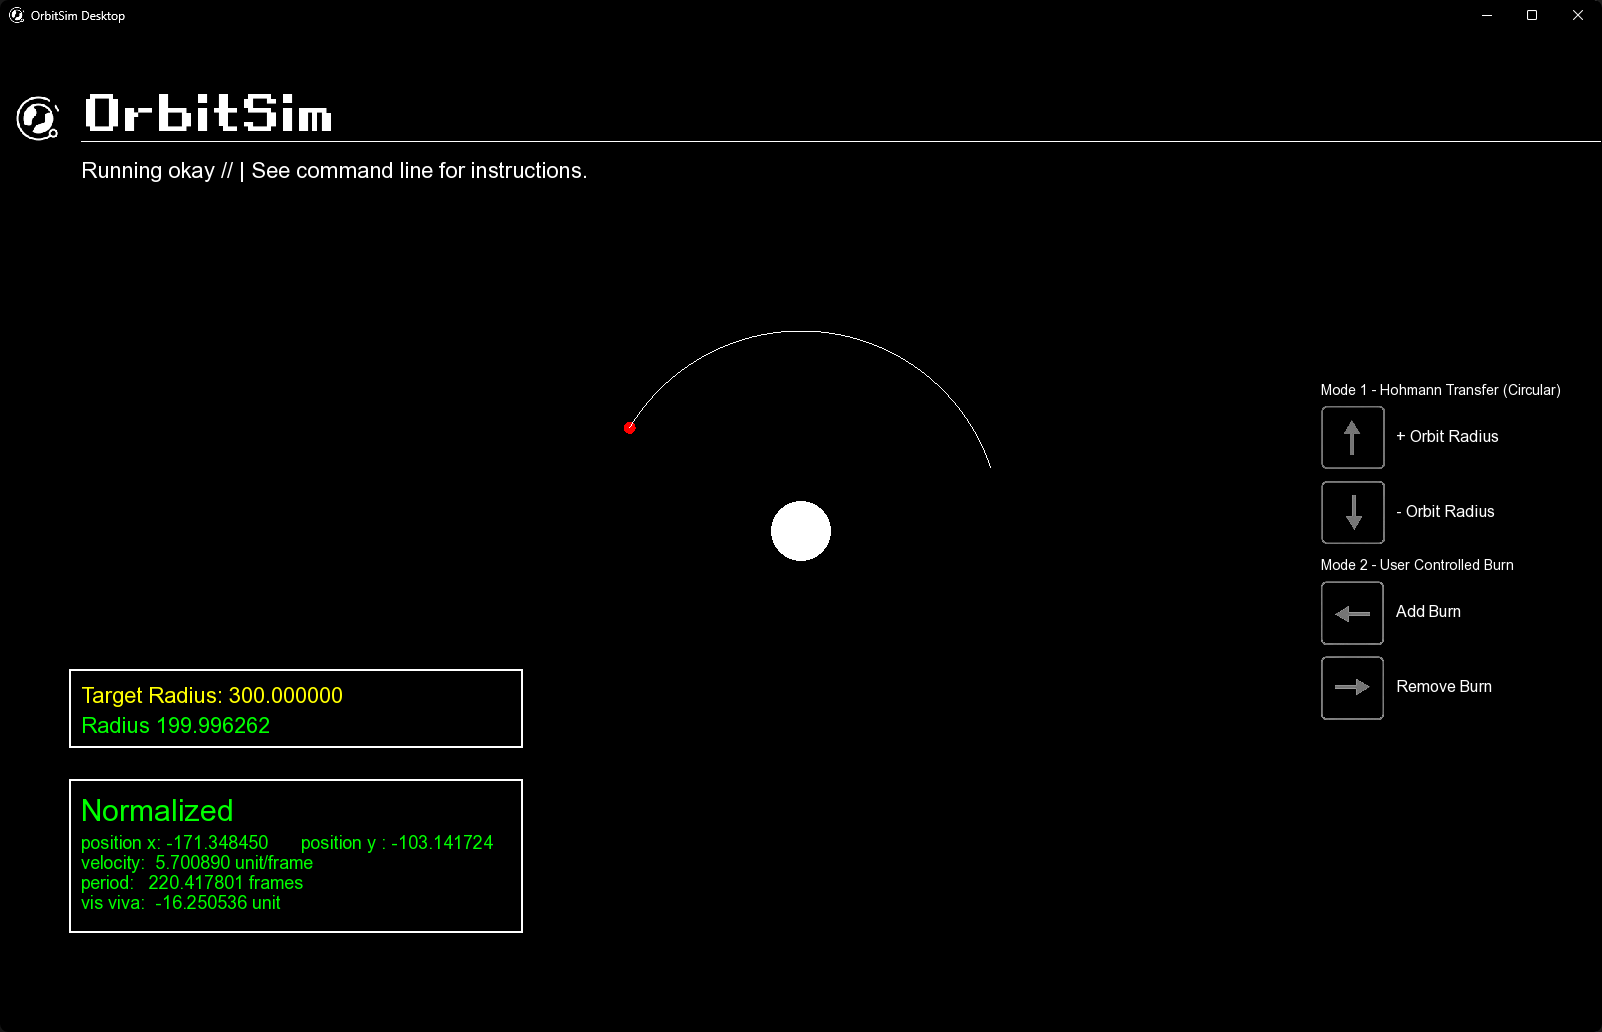
\includegraphics[width=0.99\linewidth]{figures/interface_1.png}
    \caption{Graphical User Interface - Initial State.}
    \label{fig:user_interface}
\end{figure}

\autoref{fig:transfer_orbit} illustrates the body element in an elliptical transfer orbit and \autoref{fig:target_orbit} shows the body in the final orbit defined by the user.
The real time data can be seen on the screen as well showing the current radius of the body as well as the target radius of the body. In \autoref{fig:transfer_orbit}, it can be observed that the current radius of the body is different from the target radius. Additionally, the status of the orbit transfer shows that the 2nd Hohmann transfer burn is still pending, meaning that the body is currently in the state of transfer, and in an elliptical transfer orbit. As soon as the second burn is completed, the transfer status goes back to a normal state. This can be seen in \autoref{fig:target_orbit} where the orbit radius is stable and the current readius is within the tolerance limit of the target radius.

\begin{figure}[H]
  \centering
  \begin{subfigure}{0.49\linewidth}
    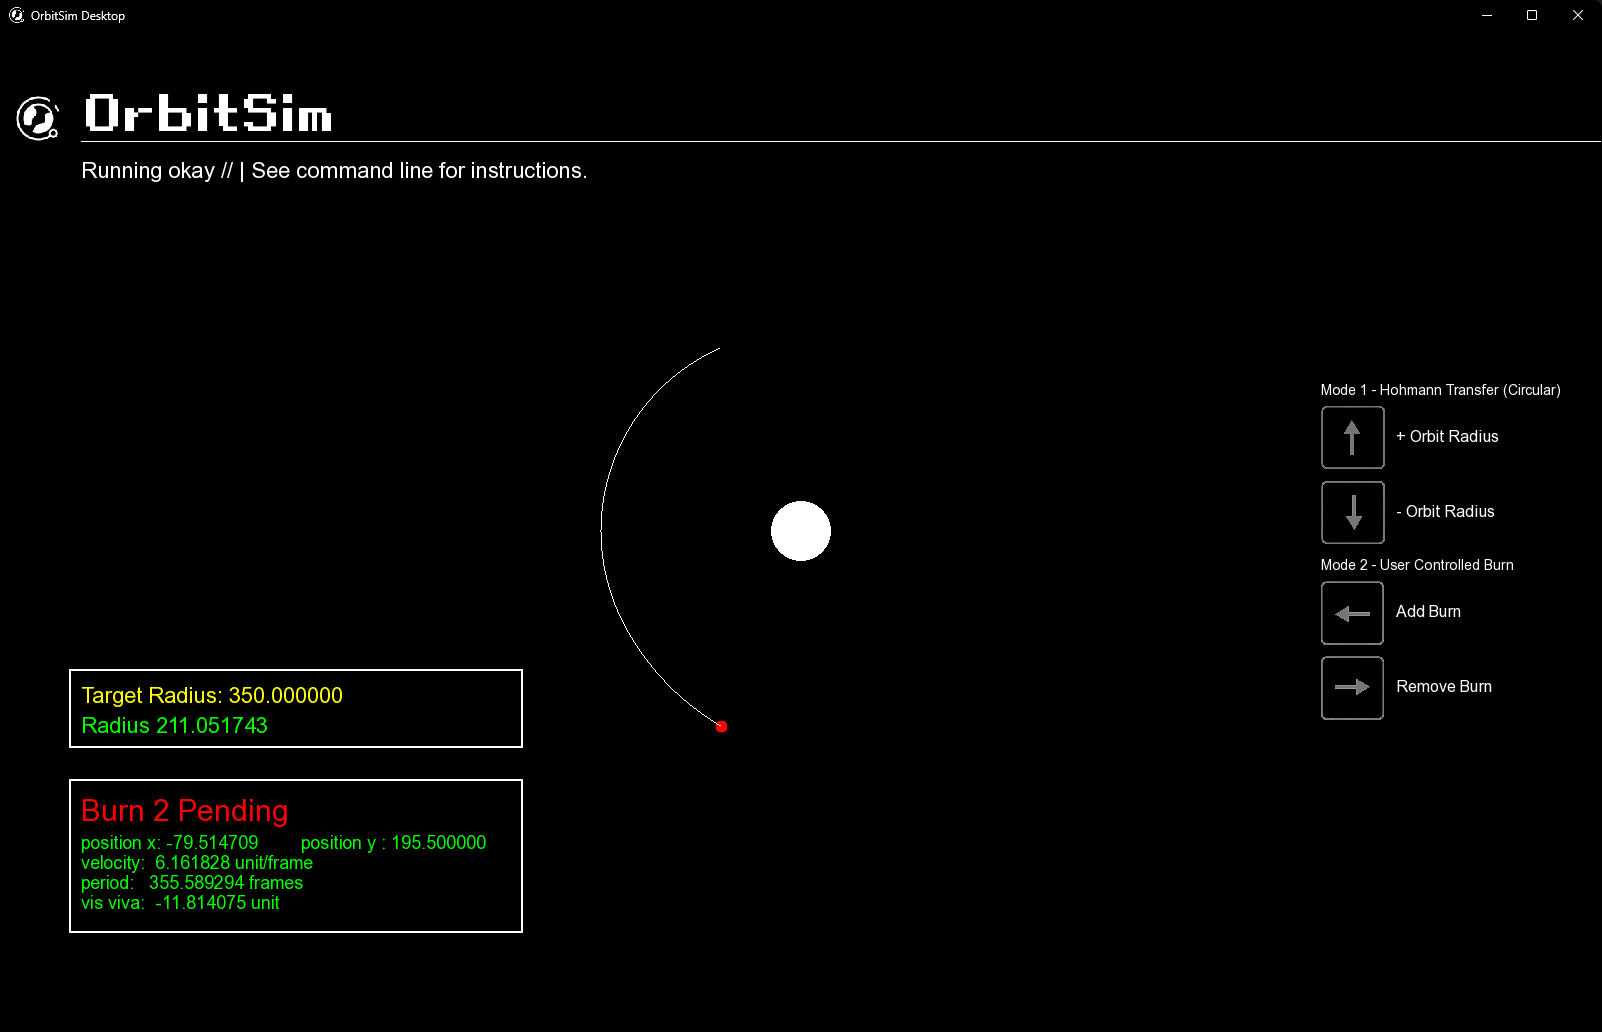
\includegraphics[width=\linewidth]{figures/transfer_state.png}
    \caption{Body in transfer orbit.}
    \label{fig:transfer_orbit}
  \end{subfigure}
  \hfill
  \begin{subfigure}{0.49\linewidth}
    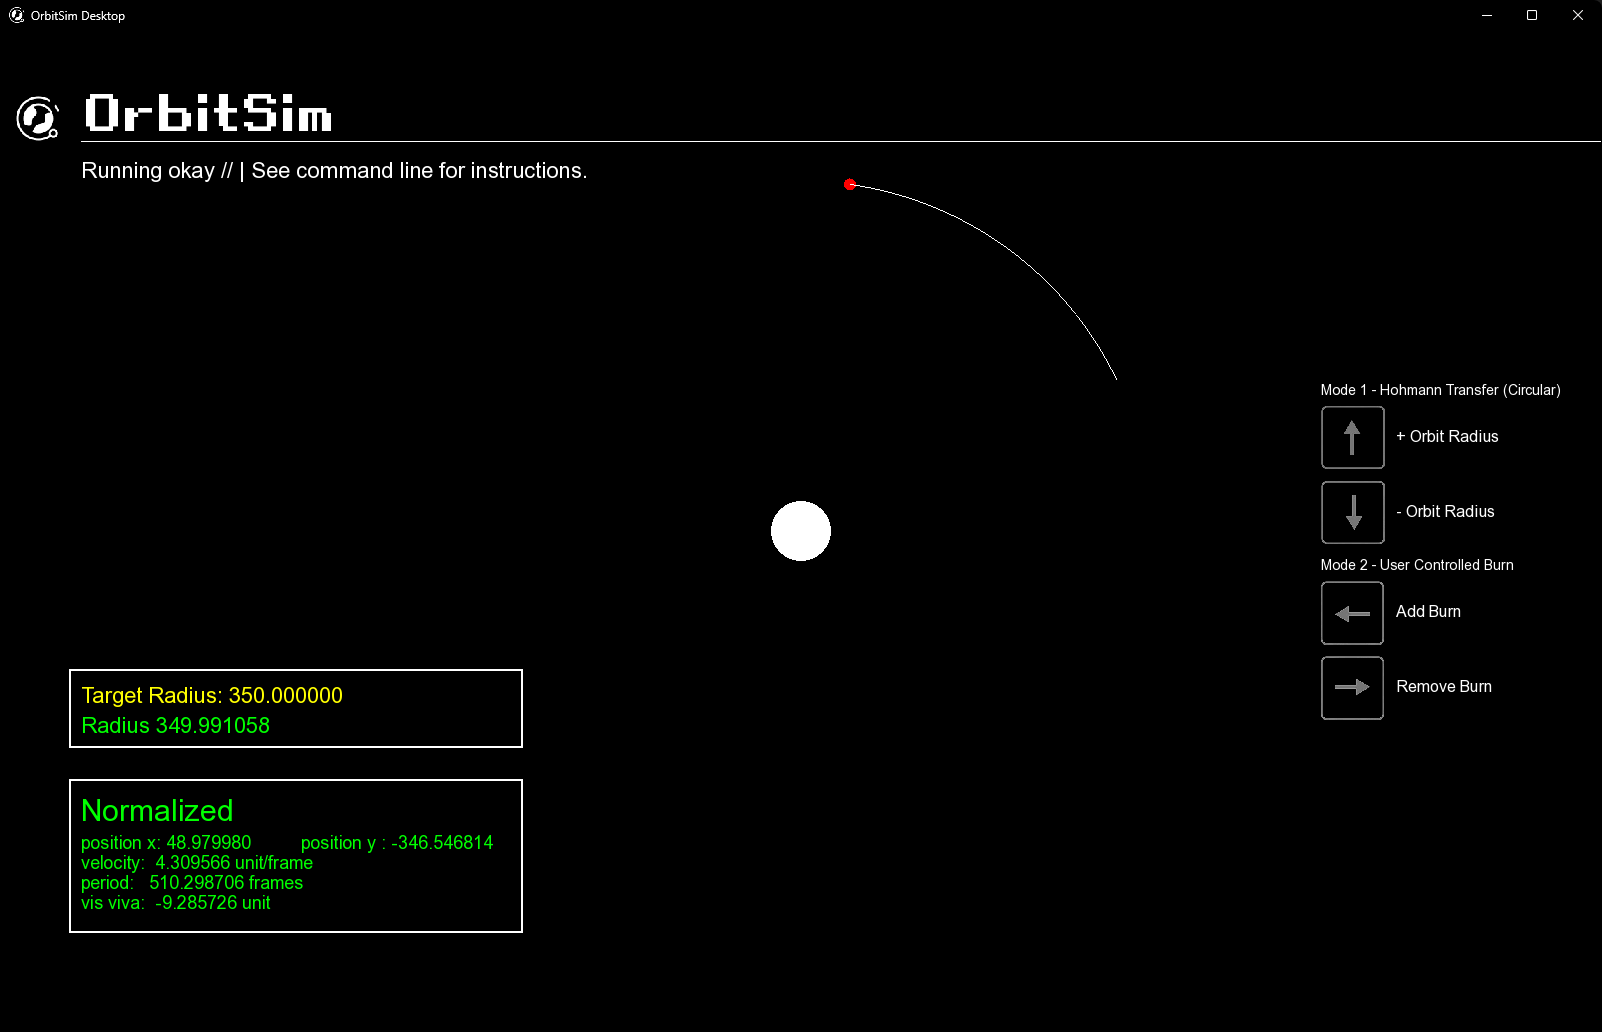
\includegraphics[width=\linewidth]{figures/final_state.png}
    \caption{Body in the user-defined target orbit.}
    \label{fig:target_orbit}
  \end{subfigure}
  

  \caption{OrbitSim showing different transfer phases.}
  \label{fig:stages}
\end{figure}

\autoref{fig:instructions} show the instructions that are printed in the console window of the desktop application for a new user to understand the functionality.

\begin{figure}[H]
        \begin{minted}[frame=lines,fontsize=\footnotesize,linenos]{cpp}
    << "INSTRUCTIONS\n"
    << "---------------------------------------  \n"
    << "Mode 1  \n"
    << "Up arrow key to increase the target orbit radius.\n"
    << "Down arrow key to decrease the target orbit radius.\n"
    << "Press T to initiate orbit transfer in Mode 1 \n"
    << "Circular orbit is required for Mode 1\n"
    << "---------------------------------------- \n"
    << "Mode 2  \n"
    << "Left arrow key to burn prograde\n"
    << "Right arrow key to burn retrograde\n"
    << "Press the spacebar key to normalize the satellite to a circular orbit. \n"
    << "---------------------------------------  \n"
    << "Ctrl + scroll wheel for zooming in and zooming out. \n"
    << "Press R to reset the orbit. \"
    << "======================================== \n";
\end{minted}
\caption{Instructions as printed in the OrbitSim desktop application console window.}
\label{fig:instructions}
\end{figure}

\clearpage



\section{Discussion}
During the development of the software, due to the limitation of the library function and knowledge gap, some change and concession are made to maintain the core function of the software. the details are discussed in the following paragraph. 

\subsection{Limitations}

The following subsections discuss the limitations of the project as well as the lessons learned while developing the desktop application.
\subsubsection{SFML Library Event Limitation}
Initially, The  is envisioned to take direct user input to set the initial condition and target orbit heights, but due to the limitation of the SFML library, this cannot be achieved. The SFML library allows the system to detect keyboard and mouse action, but user can only input value as strings which requires more manipulation to detect and filter user input error; Therefore for the robustness of the software, it is deemed a worth trade off for users to use keystrokes to manipulate target orbit radius as a slider. However,custom initialization of the satellite could not be achieved thus it is abandoned for the scope of the project.

\subsubsection{Frame Capture Performance}
During testing it is found that the sometime the software could not capture the exact frame when an action is require. Initially the basing physics on frame rate was suspected to be cause of the problem and after the decoupling time and frame rate; the problem remained. with limited time it is deemed to be acceptable to widen the acceptable range of the frame; therefore the action could be performance more reliably. However, this introduces error into the transferring action and the error caused by this are discussed in the subsequent sections.


\subsection{Error}

As mentioned in the theory section, the direct integration method assumes the time step is sufficiently small that the error accumulated between each step is negligible. However, in practice the deviation caused by this error seems to be under estimated. Attempts are made to develop a higher order governing equations to reduce the accumulated error; but in practice, the development of such equation proves to be challenging to implement. Thus the direct integration method is kept; the error causes three performance problems that are discussed below.

\subsubsection{Imperfect Initialization}
    When the satellite is initialized, even with the mathematically correct condition; the first step of the integration will cause the satellite deviate slightly as the acceleration of the first time step causes the path of the satellite to become an secant line rather than tangent. as a result, orbit shape of the satellite is slightly compressed. To mitigate this issue, the time step size massively reduce and the current radius deviation is below 0.1 unit;this deviation is deemed acceptable for the time limitation of the project.

\subsubsection{Orbit accuracy close to the gravity source}
    When the satellite is sufficiently close to the gravity source, the fidelity of the orbit suffers. As the distance between the gravity source and the satellite reduces, the gravitational pull and acceleration increases dramatically. For the same time step size, the velocity and the position covered between each time step increased as well. Due to this effect, the tangent path of the satellite taken causes the satellite to drift away from it's initial orbit. To mitigate this effect, the lowest transferable orbit radius is set to 150 unit from the center to avoid the effect, but user can still place the satellite at lower orbit manually.

\subsubsection{Transfer $\Delta$V error and correction}
    Due to the first error and the frame capture problem discussed eariler, the circularized orbit is not a perfect, therefore when calculating and performing the Hohmann transfer, very small increase of the $\Delta$V is added to compensate for the small difference caused by the imperfect orbit and after the second burn is completed; a small velocity trim is performed to reduce the error accumulated while performing the transfer.



\subsection{Lessons Learned}
This project has provided an opportunity to practice and utilize C++ language and learn the functions of the SFML development tool.  While working on this project, the structure and function of the SFML library created many unique problem related to desired function of the program and many alternative routes and solutions are explored to either solve or bypass the issue. 
For, example in the early version of the code, the software had problem triggering event after a keystroke is registered. Many modifications were made to the boolean logic of the event but to problem remained. After two days of work it is found in the documentation that frame based logic must not be placed in the event loop for the the trigger to be reliable. It is suspected that due to the compiling method used my the SFML development kit that to optimise performance, the event loop is only active when input is detected. Thus keeping the boolean logic inside the event loop will cause it to be skipped from the main loop if at the triggering time no other user inputs are made to the program. However, the triggering condition still need to we widened to compensate for the frame capturing performance.
Many similar problems were encountered during the development and some feature such as custom initialization are abandoned due to knowledge gaps. Overall this project is a valuable experience to review c++ programming and experience software design. The developed software met the expectation of the requirement.

\clearpage

\section{Conclusion}

The development of OrbitSim led to the exploration of some key theories in orbital mechanics and the understanding of a two body universe. Different methodologies have been used to write the code which provides the users with a graphical user interface to understand how orbital mechanics functions.
OrbitSim provides a platform for users to simulate orbital paths and manage various parameters effectively. The software's ability to visualize orbital transfers, manage burns, demonstrates its utility in space mission planning and analysis.

Moving forward, potential enhancements could focus on expanding the software's capabilities, improving user interface elements, and addressing any identified limitations. Overall, OrbitSim stands as a valuable tool for students and professors in the aerospace industry to explore and understand orbital mechanics in a simulated environment.

\clearpage
%%%%%%%%%%%%%%%%%%%%%%%%%%%%%%%%%%%%%%%%%%%%%%%%%%%%%%%%%%%%%%%%%%%%%%%%%%%%%%%%%%%%%%%%%%
%               REFERENCES              %
%%%%%%%%%%%%%%%%%%%%%%%%%%%%%%%%%%%%%%%%%%%%%%%%%%%%%%%%%%%%%%%%%%%%%%%%%%%%%%%%%%%%%%%%%%%
%\bibliographystyle{plain}
%\bibliography{refs}
%\pagebreak
%%%%%%%%%%%%%%%%%%%%%%%%%%%%%%%%%%%%%%%%%%%%%%%%%%%%%%%%%%%%%%%%%%%%%%%%%%%%%%%%%%%%%%%%%%
%               APPENDICES              %
%%%%%%%%%%%%%%%%%%%%%%%%%%%%%%%%%%%%%%%%%%%%%%%%%%%%%%%%%%%%%%%%%%%%%%%%%%%%%%%%%%%%%%%%%%
\appendix
\section*{APPENDICES}
\addcontentsline{toc}{section}{Appendices}

\section{OrbitSim Source Code} \label{sec:orbi_code}
\begin{minted}[frame=lines,fontsize=\footnotesize,linenos]{cpp}
#include "SFML/Graphics.hpp"
#include <vector>
#include <iostream>
#include <cmath>


class GravitySource
{
	sf::Vector2f pos;
	sf::Vector2f pos_e;
	float strength;
	sf::CircleShape s;
	sf::Texture texture_earth;

public:
	GravitySource(float pos_x, float pos_y, float strength) {
		pos.x = pos_x;
		pos.y = pos_y;
		this->strength = strength;
		pos_e.x = pos_x - 30;
		pos_e.y = pos_y - 30;

		s.setTexture(&texture_earth);
		s.setPosition(pos_e);
		s.setRadius(30);
	}

	void render(sf::RenderWindow& wind)
	{
		wind.draw(s);
	}
	sf::Vector2f get_pos()
	{
		return pos;
	}
	float get_strength()
	{
		return strength;
	}


};

class Particle {
	sf::CircleShape s;
	std::vector<sf::Vector2f> path;

public:
	sf::Vector2f pos;
	sf::Vector2f vel;
	sf::Vector2f pos_s;

	Particle(float pos_x, float pos_y, float vel_x, float vel_y) {
		pos.x = pos_x;
		pos.y = pos_y;
		pos_s.x = pos.x - 6;
		pos_s.y = pos.y - 6;
		vel.x = vel_x;
		vel.y = vel_y;

		s.setPosition(pos_s);
		s.setFillColor(sf::Color::Red);
		s.setRadius(6);
	}

	void render(sf::RenderWindow& wind) {
		s.setPosition(pos_s);
		wind.draw(s);

		// Render the path as dotted lines
		for (size_t i = 1; i < path.size(); ++i) {
			sf::Vertex line[] = {
				sf::Vertex(path[i - 1], sf::Color::White),
				sf::Vertex(path[i], sf::Color::White)
			};
			wind.draw(line, 2, sf::Lines);
		}
	}

	void set_color(sf::Color col) {
		s.setFillColor(col);
	}

	void update_physics(GravitySource& s, float dt) {
		float distance_x = s.get_pos().x - pos.x;
		float distance_y = s.get_pos().y - pos.y;

		float distance = sqrt(distance_x * distance_x + distance_y * distance_y);

		float inverse_distance = 1.f / distance;

		float normalized_x = inverse_distance * distance_x;
		float normalized_y = inverse_distance * distance_y;

		float inverse_square_dropoff = inverse_distance * inverse_distance;

		float acceleration_x = normalized_x * s.get_strength() * inverse_square_dropoff;
		float acceleration_y = normalized_y * s.get_strength() * inverse_square_dropoff;

		vel.x += acceleration_x * dt;
		vel.y += acceleration_y * dt;

		pos.x += vel.x * dt;
		pos.y += vel.y * dt;
		pos_s.x = pos.x - 6;
		pos_s.y = pos.y - 6;
		path.push_back(pos);
		// Limit the size of the path to prevent it from growing indefinitely
		if (path.size() > 20000)
			path.erase(path.begin()); // Remove the oldest position
	}
};



int main() {

std::cout << "MIT License\n"
<< "\n"
<< "Copyright (c) 2024 | Paramvir Singh Lobana | Jian Jiao\n"
<< "\n"
<< "Permission is hereby granted, free of charge, to any person obtaining a copy\n"
<< "of this software and associated documentation files (the \"Software\"), to deal\n"
<< "in the Software without restriction, including without limitation the rights\n"
<< "to use, copy, modify, merge, publish, distribute, sublicense, and/or sell\n"
<< "copies of the Software, and to permit persons to whom the Software is\n"
<< "furnished to do so, subject to the following conditions:\n"
<< "\n"
<< "The above copyright notice and this permission notice shall be included in all\n"
<< "copies or substantial portions of the Software.\n"
<< "\n"
<< "====================================================================================== \n"
<< "INSTRUCTIONS\n"
<< "-------------------------------------------------------------------------------------- \n"
<< "Mode 1  \n"
<< "Up arrow key to increase the orbit radius.\n"
<< "Down arrow key to decrease the orbit radius.\n"
<< "Press T to initiate orbit transfer in Mode 1 \n"
<< "-------------------------------------------------------------------------------------- \n"
<< "Mode 2  \n"
<< "Left arrow key \n"
<< "Right arrow key \n"
<< "Press the spacebar key to normalize the orbit in Model 2 \n"
<< "-------------------------------------------------------------------------------------- \n"
<< "Ctrl + scroll wheel for zooming in and zooming out. \n"
<< "====================================================================================== \n";


// GUI Values
float win_x = 1600;
float win_y = 1000;
float info_x = win_x * 0.05;
float info_y = win_y * 0.7;
float info_char_size = 14 + 4;

sf::RenderWindow window(sf::VideoMode(win_x, win_y), "OrbitSim Desktop");
window.setFramerateLimit(60);
sf::View view = window.getView();

// Initialize sources and particles
std::vector<GravitySource> sources;
sources.push_back(GravitySource(win_x / 2, win_y / 2, 6500));


float particle_x_start = win_x / 2 + 200;
float particle_y_start = win_y / 2;
float particle_start = sqrt(pow(200, 2) + pow(0, 2));
std::vector<Particle> particles;
particles.push_back(Particle(particle_x_start, particle_y_start,
(particle_y_start - win_y / 2) / particle_start * sqrt(6500 / particle_start), 
-(particle_x_start - win_x / 2) / particle_start * sqrt(6500 / particle_start)));

sf::Font font;
if (!font.loadFromFile("resources\\arial.ttf")) {
std::cerr << "Failed to load font file!\n";
return EXIT_FAILURE;
}
sf::Font font_orb;
if (!font_orb.loadFromFile("resources\\retro_gaming.ttf")) {
std::cerr << "Failed to load font file!\n";
return EXIT_FAILURE;
}

// setup output
sf::Text orbitsim;
sf::Text status_string;
sf::Text velocity;
sf::Text position2; sf::Text position1; sf::Text Radius;
sf::Text period;
sf::Text vis_viva;
sf::Text plus;
sf::Text minus;
sf::Text tsf;
sf::Text Target_Orbit;

// Display value
// float P_x = particles[0].pos.x;
float P_x = 0;
float P_y = 0;
float t = 1.f;
float V_abs = 0;
float Dv_1 = 0;
float Dv_2 = 0;
float P_abs = 0;
float P_abs_tf = 0;
float E_cond = 0;
float P_cond = 0;
float Target_O = 300;
int i = 3;


float timeScale = 20.0f; // Defines how fast the particle is running

sf::Clock clock;
const float fixedTimeStep = 1.0f / 5000.0f; // 60 FPS


// Add program icon
sf::Image icon;
icon.loadFromFile("resources\\orb.png");
window.setIcon(icon.getSize().x, icon.getSize().y, icon.getPixelsPtr());

//define key parameters
float key_pos_x = 0.825; float key_pos_y = 5;
float key_scale_val = 0.6;

// Add key image
sf::Text m_1; m_1.setFont(font); m_1.setString("Mode 1 - Hohmann Transfer (Circular)"); m_1.setCharacterSize(14); m_1.setPosition(win_x * key_pos_x, win_y * 0.375 - 25);
sf::Text m_11; m_11.setFont(font); m_11.setString("+ Orbit Radius");
m_11.setCharacterSize(16); m_11.setPosition(win_x * key_pos_x + 75, win_y * 0.375 + 20);
sf::Text m_12; m_12.setFont(font); m_12.setString("- Orbit Radius");
m_12.setCharacterSize(16); m_12.setPosition(win_x * key_pos_x + 75, win_y * 0.45 + 20);
sf::Texture keys_up; sf::Sprite up_key;
if (!keys_up.loadFromFile("resources\\key_up.png"))
std::cout << "Error loading the image ... " << std::endl;
up_key.setTexture(keys_up); up_key.setPosition
(sf::Vector2f(win_x * key_pos_x, win_y * 0.375)); up_key.setScale(key_scale_val, key_scale_val);


sf::Texture keys_down; sf::Sprite down_key;
if (!keys_down.loadFromFile("resources\\key_down.png")) std::cout << "Error loading the image ... " << std::endl;
down_key.setTexture(keys_down); down_key.setPosition(sf::Vector2f(win_x * key_pos_x, win_y * 0.45)); down_key.setScale(key_scale_val, key_scale_val);

sf::Text m_2; m_2.setFont(font); m_2.setString("Mode 2 - User Controlled Burn"); m_2.setCharacterSize(14); m_2.setPosition(win_x * key_pos_x, win_y * 0.55 - 25);
sf::Text m_21; m_21.setFont(font); m_21.setString("Add Burn"); m_21.setCharacterSize(16); m_21.setPosition(win_x * key_pos_x + 75, win_y * 0.55 + 20);
sf::Text m_22; m_22.setFont(font); m_22.setString("Remove Burn"); m_22.setCharacterSize(16); m_22.setPosition(win_x * key_pos_x + 75, win_y * 0.625 + 20);
sf::Texture keys_l; sf::Sprite left_key;
if (!keys_l.loadFromFile("resources\\key_left.png"))
std::cout << "Error loading the image ... " << std::endl;
left_key.setTexture(keys_l); left_key.setPosition
(sf::Vector2f(win_x * key_pos_x, win_y * 0.55)); left_key.setScale(key_scale_val, key_scale_val);

sf::Texture keys_r; sf::Sprite right_key;
if (!keys_r.loadFromFile("resources\\key_right.png"))
std::cout << "Error loading the image ... " << std::endl;
right_key.setTexture(keys_r); right_key.setPosition
(sf::Vector2f(win_x * key_pos_x, win_y * 0.625)); right_key.setScale(key_scale_val, key_scale_val);

sf::Texture logo; sf::Sprite logo_orb;
if (!logo.loadFromFile("resources\\orb.png")) 
std::cout << "Error loading the image ... " << std::endl;
logo_orb.setTexture(logo); logo_orb.setPosition
(sf::Vector2f(15, win_y * 0.05 + 15)); logo_orb.setScale(0.7, 0.7);

while (window.isOpen()) {
sf::Time deltaTime = clock.restart();
float accumulator = deltaTime.asSeconds();
float dt = std::min(accumulator, fixedTimeStep);

while (accumulator > 0) {

// Handle events
sf::Event event;

P_x = particles[0].pos.x;
P_y = particles[0].pos.y;
P_abs = sqrt(pow(P_x - win_x / 2, 2) + pow(P_y - win_y / 2, 2));
// calcuate for tangency 
float V_x = particles[0].vel.x;
float V_y = particles[0].vel.y;
V_abs = sqrt(pow(V_x, 2) + pow(V_y, 2));

while (window.pollEvent(event))

{
    if (event.type == sf::Event::Closed)
        window.close();

    if (sf::Keyboard::isKeyPressed(sf::Keyboard::Escape))
        window.close();




    // Manual input of control
    if (sf::Keyboard::isKeyPressed(sf::Keyboard::Left) && i != 0 && i != 1)
    {
        // tangent burn
        particles[0].vel.x += 0.1f * V_x / V_abs;
        particles[0].vel.y += 0.1f * V_y / V_abs;
        i = 10;
    }
    else if (sf::Keyboard::isKeyPressed(sf::Keyboard::Right) && i != 0 && i != 1)
    {
        particles[0].vel.x -= 0.1f * V_x / V_abs;
        particles[0].vel.y -= 0.1f * V_y / V_abs;
        i = 10;
    }

    // Nornalize based on altitude

    if (sf::Keyboard::isKeyPressed(sf::Keyboard::Space))
    {
        particles[0].vel = sf::Vector2f((P_y - win_y / 2) / P_abs
* sqrt(6500 / P_abs), -(P_x - win_x / 2) / P_abs * sqrt(6500 / P_abs));
        i = 3;

    }


    else if (sf::Keyboard::isKeyPressed(sf::Keyboard::Up) && i != 0 && i != 1)


    {
        if (Target_O < 350)
            Target_O++;
    }


    else if (sf::Keyboard::isKeyPressed(sf::Keyboard::Down) && i != 0 && i != 1)


    {
        if (Target_O > 150)
            Target_O--;
    }


    // Change velocity of the first particle if T
    if (sf::Keyboard::isKeyPressed(sf::Keyboard::T) && i == 3)
    {

        i = 0;
    }

    if (sf::Keyboard::isKeyPressed(sf::Keyboard::R))
    {
        particles[0].pos = sf::Vector2f(win_x / 2 - 200, win_y / 2);
        particles[0].vel = sf::Vector2f((particles[0].pos.y - win_y / 2) 
/ sqrt(pow(200,2)) * sqrt(6500 / pow(200, 2)), -(particles[0].pos.x - win_x / 2) 
/ sqrt(pow(200, 2)) * sqrt(6500 / sqrt(pow(200, 2))));
        i = 3;

    }

    // Zoom in

    if (event.type == sf::Event::MouseWheelScrolled && event.mouseWheelScroll.wheel == sf::Mouse::VerticalWheel)
    {
        if (sf::Keyboard::isKeyPressed(sf::Keyboard::LControl) || sf::Keyboard::isKeyPressed(sf::Keyboard::RControl))
        {
            if (event.mouseWheelScroll.delta > 0)
                view.zoom(0.9f);
            else if (event.mouseWheelScroll.delta < 0)
                view.zoom(1.1f);

            window.setView(view);
        }
    }


}

// moved outside event loop to fig mouse bug

if (i == 0)
{
    P_abs_tf = P_abs;
    Dv_1 = 1.0001 * sqrt(6500 * (2 / P_abs_tf - 2 / (P_abs_tf + Target_O)));
    Dv_2 = sqrt(6500 / Target_O);
    particles[0].vel.x = Dv_1 * V_x / V_abs;
    particles[0].vel.y = Dv_1 * V_y / V_abs;
    i = 1;
}
if (-0.2 < P_abs - Target_O && P_abs - Target_O < 0.2 && i == 1)
{
    particles[0].vel.x = Dv_2 * V_x / V_abs;
    particles[0].vel.y = Dv_2 * V_y / V_abs;
    i = 2;
}

if (-0.001 < P_abs - Target_O && P_abs - Target_O < 0.001 && i == 2)
{
    particles[0].vel = sf::Vector2f((P_y - win_y / 2) / P_abs * sqrt(6500 / P_abs), -(P_x - win_x / 2) / P_abs * sqrt(6500 / P_abs));
    i = 3;

}






// Update physics
for (auto& source : sources) {
    for (auto& particle : particles) {
        particle.update_physics(source, dt * timeScale);
        }
    }
    accumulator -= dt;
    // Render
}

window.clear();
for (auto& source : sources)
{
    source.render(window);
}
for (auto& particle : particles)
{
    particle.render(window);
}

// ==================================== PRINT SOFTWARE INFO =============================================
orbitsim.setFont(font_orb);
orbitsim.setString("OrbitSim");
orbitsim.setCharacterSize(50);
orbitsim.setFillColor(sf::Color::White);
orbitsim.setPosition(win_x * 0.05, win_y * 0.05);

status_string.setFont(font);
status_string.setString("Running okay // | See command line for instructions.");
status_string.setCharacterSize(info_char_size + 4);
status_string.setFillColor(sf::Color::White);
status_string.setPosition(win_x * 0.05, win_y * 0.05 + 75);


sf::VertexArray lines(sf::LinesStrip, 2);
lines[0].position = sf::Vector2f(win_x * 0.05, win_y * 0.11);
lines[1].position = sf::Vector2f(win_x * 1, win_y * 0.11);

sf::RectangleShape rect(sf::Vector2f(450.f, 75.f));
rect.setPosition(sf::Vector2f(info_x - 10, 650 - 10)); rect.setFillColor(sf::Color::Transparent); rect.setOutlineColor(sf::Color::White); rect.setOutlineThickness(2);

sf::RectangleShape rect2(sf::Vector2f(450.f, 150.f));
rect2.setPosition(sf::Vector2f(info_x - 10, 760 - 10)); rect2.setFillColor(sf::Color::Transparent); rect2.setOutlineColor(sf::Color::White); rect2.setOutlineThickness(2);
// ==================================== END OF SOFTWARE INFO =============================================
//===================================== START OF DATA PRINTING ==========================================
std::string t_string;
t_string = std::to_string(t);

// Display Pos

std::string P_abs_string;
P_abs_string = std::to_string(P_abs);
std::string pos_x_string;
pos_x_string = std::to_string(P_x - win_x / 2);
std::string pos_y_string;
pos_y_string = std::to_string(P_y - win_y / 2);


position1.setFont(font);
position1.setString("position x: " + pos_x_string);
position1.setCharacterSize(info_char_size);
position1.setFillColor(sf::Color::Green);
position1.setPosition(info_x, 800);

position2.setFont(font);
position2.setString("position y : " + pos_y_string);
position2.setCharacterSize(info_char_size);
position2.setFillColor(sf::Color::Green);
position2.setPosition(info_x + 220, 800);



// Display Time Period
//position.setFont(font);
//position.setString("Time: " + t_string + " s");
//position.setCharacterSize(info_char_size);
//position.setFillColor(sf::Color::Green);
//position.setPosition(info_x, 800);

// Display Vel

float V_x = particles[0].vel.x;
float V_y = particles[0].vel.y;
V_abs = sqrt(pow(V_x, 2) + pow(V_y, 2));
std::string V_abs_string;
V_abs_string = std::to_string(V_abs);

velocity.setFont(font);
velocity.setString("velocity:  " + V_abs_string + " unit/frame");
velocity.setCharacterSize(info_char_size);
velocity.setFillColor(sf::Color::Green);
velocity.setPosition(info_x, 820);
// setup velocity indication 
plus.setFont(font);
plus.setString("Prograde");
plus.setCharacterSize(info_char_size + 2);
plus.setFillColor(sf::Color::Red);
plus.setPosition(info_x + 300, 820);

minus.setFont(font);
minus.setString("Retrograde");
minus.setCharacterSize(info_char_size + 2);
minus.setFillColor(sf::Color::Red);
minus.setPosition(info_x + 300, 820);

// Display period
float a = 0;
a = 1 / ((2.0f / P_abs) - (pow(V_abs, 2) / 6500.0f));
P_cond = ((2 * 3.1415926) / sqrt(6500.0f)) * pow(a, 1.5);
std::string P_cond_string;
P_cond_string = std::to_string(P_cond);
period.setFont(font);
period.setString("period:   " + P_cond_string + " frames");
period.setCharacterSize(info_char_size);
period.setFillColor(sf::Color::Green);
period.setPosition(info_x, 840);

// display vis_viva
E_cond = pow(V_abs, 2) * 0.5f - 6500.0f / P_abs;
std::string E_cond_string;
E_cond_string = std::to_string(E_cond);

vis_viva.setFont(font);
vis_viva.setString("vis viva:  " + E_cond_string + " unit");
vis_viva.setCharacterSize(info_char_size);
if (E_cond < 0)
vis_viva.setFillColor(sf::Color::Green);
else
vis_viva.setFillColor(sf::Color::Red);
vis_viva.setPosition(info_x, 860);


if (sf::Keyboard::isKeyPressed(sf::Keyboard::Left) && i != 0 && i != 1)
window.draw(plus);

if (sf::Keyboard::isKeyPressed(sf::Keyboard::Right) && i != 0 && i != 1)
window.draw(minus);

// Display target Orb
std::string Target_O_string;
Target_O_string = std::to_string(Target_O);
Target_Orbit.setFont(font);
Target_Orbit.setString("Target Radius: " + Target_O_string);
Target_Orbit.setCharacterSize(info_char_size + 4);
Target_Orbit.setFillColor(sf::Color::Yellow);
Target_Orbit.setPosition(info_x, 650);

Radius.setFont(font);
Radius.setString("Radius " + P_abs_string);
Radius.setCharacterSize(info_char_size + 4);
Radius.setFillColor(sf::Color::Green);
Radius.setPosition(info_x, 680);

// display tsf
tsf.setFont(font);
if (i == 0)
{
tsf.setString("Burn 1");
tsf.setFillColor(sf::Color::Red);
}
if (i == 1)
{
tsf.setString("Burn 2 Pending");
tsf.setFillColor(sf::Color::Red);
}
if (i >= 2 && i < 3)
{
tsf.setString("Trim adjustment Pending");
tsf.setFillColor(sf::Color::Yellow);
}

if (i == 3)
{
tsf.setString("Normalized");
tsf.setFillColor(sf::Color::Green);
}

if (i == 10)
{
tsf.setString("Cannot transfer; Normalize");
tsf.setFillColor(sf::Color::Red);
}
tsf.setCharacterSize(30);

tsf.setPosition(info_x, 760);
// Other info to be printed


//====================================== DRAW INFORMATION ==========================================
window.draw(orbitsim);
window.draw(status_string);
window.draw(rect); window.draw(rect2);
window.draw(logo_orb);
window.draw(up_key); window.draw(down_key); window.draw(right_key); window.draw(left_key);
window.draw(m_1); window.draw(m_2); window.draw(m_11); window.draw(m_12); window.draw(m_21); window.draw(m_22);
window.draw(lines);
window.draw(tsf);
window.draw(velocity);
window.draw(position2); window.draw(position1); window.draw(Radius); window.draw(Target_Orbit);
window.draw(period);
window.draw(vis_viva);
//===================================== END OF DATA PRINTING ==========================================


window.display();

t += dt * timeScale;
}

return 0;
}
\end{minted}

\end{document}